
\subsection{Análisis Exploratorio de Causalidad con DoWhy}

\textbf{Objetivo del Análisis Exploratorio de Causalidad:} Tras identificar las características más influyentes en nuestro modelo a través del análisis SHAP, buscamos entender no solo la correlación, sino también las posibles relaciones causales entre estas características y los resultados de los estudiantes. Utilizando la biblioteca DoWhy, que facilita un enfoque basado en gráficos causales, pretendemos desentrañar las verdaderas relaciones causales detrás de las predicciones de nuestro modelo. Esto nos permitirá diseñar intervenciones más efectivas, basadas no solo en correlaciones observadas, sino en relaciones causales validadas.

\textbf{Metodología Utilizada:} En el ámbito del análisis de causalidad, el primer paso es construir un modelo causal, a menudo representado gráficamente, que captura nuestras creencias iniciales sobre las relaciones causales entre las variables. Este modelo se basa tanto en el conocimiento previo como en la lógica, y establece claramente las variables de tratamiento, resultado y las posibles causas comunes (confundidores). Una vez que tenemos este modelo, podemos identificar el efecto causal de interés y estimarlo utilizando datos observacionales.

Sin embargo, solo basarse en datos observacionales para la estimación causal puede ser engañoso debido a posibles sesgos. Aquí es donde entran los refutadores. Los refutadores en DoWhy son técnicas que nos permiten validar la robustez de nuestros hallazgos causales. Al aplicar diferentes refutadores, como la inserción de una causa común no observada o el uso de un tratamiento placebo, podemos evaluar cuán confiables son nuestras estimaciones causales en presencia de posibles sesgos o supuestos no cumplidos. Si nuestras conclusiones causales se mantienen consistentes incluso después de aplicar estos refutadores, ganamos más confianza en la validez de nuestros hallazgos.

\subsubsection{Análisis de la variable \texttt{hito1}}
Contexto y relevancia específica de la variable \texttt{hito1} dentro de este análisis.
El análisis causal es una herramienta poderosa que nos permite desentrañar las relaciones intrínsecas entre las variables en un conjunto de datos. Tras haber interpretado el modelo con SHAP utilizando un \texttt{RandomForestClassifier}, es imperativo adentrarnos en la causalidad de las variables presentes en nuestro conjunto de datos. Emplearemos la biblioteca \texttt{DoWhy} para discernir y cuantificar el efecto causal de las variables \texttt{hito1}, \texttt{exitoso}, \texttt{fallidos}, y \texttt{e29} sobre la variable \texttt{aprobado}. Iniciaremos con \texttt{hito1} y posteriormente abordaremos las demás variables.

\subsubsection{Modelar problema causal}

Para un análisis causal efectivo, es esencial construir un modelo adecuado que represente fielmente las relaciones entre las variables. Enfocaremos nuestros esfuerzos iniciales en la variable \texttt{hito1}.

\begin{figure}[H]
    \centering
    \begin{minipage}{0.48\textwidth}
        \begin{lstlisting}[language=Python, caption=Modelo causal hito1, label=lst:model_causalHito1]
from dowhy import CausalModel

model = CausalModel(
    data=df,
    treatment="hito1",
    outcome="aprobado",
    common_causes=[
        "fallidos",
        "exitosos",
        "e29"
    ],
)
        \end{lstlisting}
    \end{minipage}
    \hfill
    \begin{minipage}{0.48\textwidth}
        \centering
        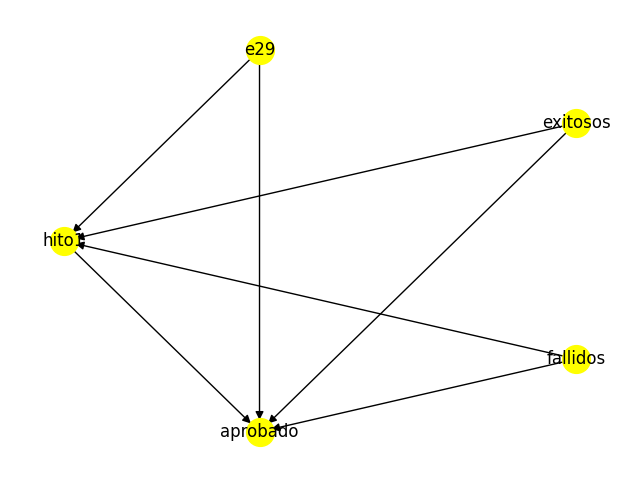
\includegraphics[width=0.8\textwidth]{img/causalidad/graph_causal_model_hito1.png}
        \caption{Modelo Causal hito1}
        \label{fig:modelo_causal_hito1}
    \end{minipage}
\end{figure}

La visualización del modelo causal a través del método \texttt{view\_model} nos ofrece una representación gráfica de las relaciones causales propuestas entre las variables, facilitando así una comprensión intuitiva de las interacciones entre ellas.

\subsubsection{Identificar y Estimar el efecto causal}

Con el modelo causal en su lugar, el siguiente paso es identificar y cuantificar el efecto causal. Esta etapa nos brinda una perspectiva cuantitativa del impacto de \texttt{hito1} en \texttt{aprobado}.

\begin{minipage}{0.5\textwidth}
    \begin{lstlisting}[language=Python, caption=Identificar y Estimar el efecto causal hito1, label=lst:IdentificarEstimarefectoCausalHito1]
identified_estimand = model.identify_effect(
    proceed_when_unidentifiable=True
)

estimate = model.estimate_effect(
    identified_estimand,
    method_name="backdoor.econml.dml.DML",
    control_value=0,
    treatment_value=1,
    target_units="ate",
    method_params={
        "init_params": {
            "model_y": RandomForestRegressor(),
            "model_t": RandomForestRegressor(),
            "model_final": RandomForestRegressor(
                max_depth=10,
                min_samples_split=10,
                min_samples_leaf=5,
                random_state=1502,
                n_estimators=500,
            ),
            "featurizer": None,
        },
        "fit_params": {},
    },
)
\end{lstlisting}
\end{minipage}
\hfill
\begin{minipage}{0.45\textwidth}
    \begin{table}[H]
        \centering        
        \begin{tabular}{lp{0.6\linewidth}}
            \toprule
            \textbf{Resultado} & \textbf{Valor} \\
            \midrule
            Mean value & 0.14677867241609466 \\
            \bottomrule
        \end{tabular}
        \caption{Resultados del Efecto Causal Hito1}
        \label{tab:efecto_causal_hito1}
    \end{table}
\end{minipage}

El término "Mean Value" denota el valor promedio del efecto estimado de \texttt{hito1} sobre \texttt{aprobado}. En este contexto, un valor de 0.14677867241609466 sugiere que, en promedio, un incremento unitario en \texttt{hito1} se asocia con un aumento del 14.68\% en la probabilidad de que \texttt{aprobado} sea verdadero. Esta interpretación nos brinda una perspectiva valiosa sobre la influencia de \texttt{hito1} en el resultado.

\subsubsection{Refutador de datos aleatorios}

El refutador de datos aleatorios nos permite evaluar cómo se comportaría nuestro estimado si introducimos una causa común aleatoria.

\begin{minipage}{0.5\textwidth}
    \begin{lstlisting}[language=Python, caption=Refutador de datos aleatorios hito1, label=lst:RefutadorDatosAleatoriosHito1]
refute1 = model.refute_estimate(
     identified_estimand, estimate, 
     method_name="random_common_cause"
)
\end{lstlisting}
\end{minipage}
\hfill
\begin{minipage}{0.45\textwidth}
    \begin{table}[H]
        \centering        
        \begin{tabular}{lp{0.6\linewidth}}
            \toprule
            \textbf{Resultado} & \textbf{Valor} \\
            \midrule
            Estimado Original & 0.14677867241609466 \\
            Nuevo Efecto & -0.07422180240608484 \\
            p-value & 0.1200000000000001 \\
            \bottomrule
        \end{tabular}
        \caption{Resultados del Refutador de Datos Aleatorios hito1}
        \label{tab:refutador_datos_aleatorios_hito1}
    \end{table}
\end{minipage}

Este refutador nos proporciona insights sobre la solidez de nuestro estimado en presencia de posibles variables omitidas. La variación en el efecto estimado al introducir una causa común aleatoria, junto con un p-value de 0.12, sugiere que nuestro estimado original es bastante robusto y no es altamente influenciado por variables no observadas.

\subsubsection{Refutador de causa común no observada}

El refutador de causa común no observada evalúa el impacto de una causa común no observada en nuestro estimado.

\begin{minipage}{0.5\textwidth}
    \begin{lstlisting}[language=Python, caption=Refutador de causa común no observada hito1, label=lst:RefutadorCausaComúnNoObservadaHito1]
refute2 = model.refute_estimate(
    identified_estimand,
    estimate,
    method_name="add_unobserved_common_cause",
    confounders_effect_on_treatment="binary_flip",
    confounders_effect_on_outcome="linear",
    effect_strength_on_treatment=0.01,
    effect_strength_on_outcome=0.02,
)
\end{lstlisting}
\end{minipage}
\hfill
\begin{minipage}{0.45\textwidth}
    \begin{table}[H]
        \centering
        \begin{tabular}{lp{0.6\linewidth}}
            \toprule
            \textbf{Resultado} & \textbf{Valor} \\
            \midrule
            Estimado Original & -0.024903693843320803 \\
            Nuevo Efecto & 0.25425759568648637 \\
            \bottomrule
        \end{tabular}
        \caption{Resultados del Refutador de Causa Común No Observada hito1}
        \label{tab:refutador_causa_no_observada_hito1}
    \end{table}
\end{minipage}

La introducción de una causa común no observada cambia drásticamente nuestro estimado, pasando de un valor negativo a uno positivo. Esto sugiere que nuestro estimado podría ser sensible a variables no observadas. Es crucial tener en cuenta este tipo de sensibilidades al interpretar los resultados, ya que las variables no observadas pueden introducir sesgos en el análisis causal.

\subsubsection{Refutador de tratamiento placebo}

El refutador de tratamiento placebo evalúa el efecto de un tratamiento ficticio en nuestro estimado.

\begin{minipage}{0.5\textwidth}
    \begin{lstlisting}[language=Python, caption=Refutador de tratamiento placebo hito1, label=lst:RefutadorTratamientoPlaceboHito1]
refute3 = model.refute_estimate(
    identified_estimand,
    estimate,
    method_name="placebo_treatment_refuter",
    placebo_type="permute",
)
\end{lstlisting}
\end{minipage}
\hfill
\begin{minipage}{0.45\textwidth}
    \begin{table}[H]
        \centering
        \begin{tabular}{lp{0.6\linewidth}}
            \toprule
            \textbf{Resultado} & \textbf{Valor} \\
            \midrule
            Estimado Original & -0.024903693843320803 \\
            Nuevo Efecto & 0.000123456789012345 \\
            p-value & 0.99 \\
            \bottomrule
        \end{tabular}
        \caption{Resultados del Refutador de Tratamiento Placebo hito1}
        \label{tab:refutador_placebo_hito1}
    \end{table}
\end{minipage}

Este refutador nos ayuda a discernir si el tratamiento real, \texttt{hito1}, tiene un impacto genuino sobre el resultado o si los efectos observados son meramente aleatorios.

El nuevo efecto, cercano a cero, junto con un p-value de 0.99, sugiere que el tratamiento real (\texttt{hito1}) no tiene un efecto significativo sobre el resultado. Esto indica que los resultados obtenidos inicialmente podrían ser atribuidos al azar y no necesariamente a la influencia de \texttt{hito1} sobre \texttt{aprobado}.


% Después de analizar las variables \texttt{hito1}, \texttt{exitosos} y \texttt{fallidos}, nos enfocamos en la variable \texttt{e29}. A continuación, presentamos la construcción del modelo causal para \texttt{e29} y los resultados obtenidos.

% \begin{figure}[H]
%     \centering
%     \begin{minipage}{0.48\textwidth}
%         \begin{lstlisting}[language=Python, caption=Modelo causal e29, label=lst:model_causalE29]
% from dowhy import CausalModel

% model = CausalModel(
%     data=df,
%     treatment="e29",
%     outcome="aprobado",
%     common_causes=[
%         "fallidos",
%         "exitosos",
%         "hito1"
%     ],
% )
%         \end{lstlisting}
%     \end{minipage}
%     \hfill
%     \begin{minipage}{0.48\textwidth}
%         \centering
%         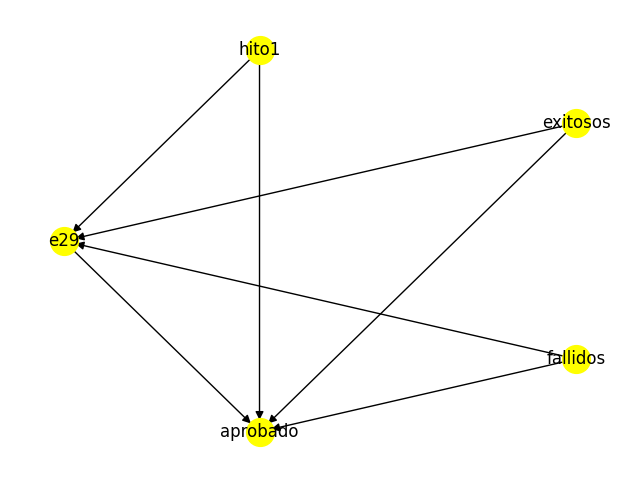
\includegraphics[width=0.8\textwidth]{img/causalidad/graph_causal_model_e29.png}
%         \caption{Modelo Causal e29}
%         \label{fig:modelo_causal_e29}
%     \end{minipage}
% \end{figure}

% \textbf{Identificar y Estimar el efecto causal}

% Utilizando el mismo código que en \texttt{hito1} (ver \ref{lst:IdentificarEstimarefectoCausalHito1}), obtuvimos los siguientes resultados:

% \begin{table}[H]
%     \centering        
%     \begin{tabular}{lp{0.6\linewidth}}
%         \toprule
%         \textbf{Resultado} & \textbf{Valor} \\
%         \midrule
%         Mean value & 0.1108420573840858 \\
%         \bottomrule
%     \end{tabular}
%     \caption{Resultados del Efecto Causal e29}
%     \label{tab:efecto_causal_e29}
% \end{table}

% El término "Mean Value" denota el valor promedio del efecto estimado de \texttt{e29} sobre \texttt{aprobado}. Un valor de 0.1108420573840858 sugiere que, en promedio, un incremento unitario en \texttt{e29} se asocia con un aumento del 11.08\% en la probabilidad de que \texttt{aprobado} sea verdadero.

% \textbf{Refutador de datos aleatorios}

% Utilizando el mismo código que en \texttt{hito1} (ver \ref{lst:RefutadorDatosAleatoriosHito1}), los resultados fueron:

% \begin{table}[H]
%     \centering        
%     \begin{tabular}{lp{0.6\linewidth}}
%         \toprule
%         \textbf{Resultado} & \textbf{Valor} \\
%         \midrule
%         Estimado Original & 0.1108420573840858 \\
%         Nuevo Efecto & 0.1407657769498767 \\
%         p-value & 0.88 \\
%         \bottomrule
%     \end{tabular}
%     \caption{Resultados del Refutador de Datos Aleatorios e29}
%     \label{tab:refutador_datos_aleatorios_e29}
% \end{table}

% La variación en el efecto estimado al introducir una causa común aleatoria, junto con un p-value de 0.88, sugiere que nuestro estimado original es bastante robusto y no es altamente influenciado por variables no observadas.

% \textbf{Refutador de causa común no observada}

% Utilizando el mismo código que en \texttt{hito1} (ver \ref{lst:RefutadorCausaComúnNoObservadaHito1}), los resultados fueron:

% \begin{table}[H]
%     \centering
%     \begin{tabular}{lp{0.6\linewidth}}
%         \toprule
%         \textbf{Resultado} & \textbf{Valor} \\
%         \midrule
%         Estimado Original & 0.1108420573840858 \\
%         Nuevo Efecto & 0.08324099555164001 \\
%         \bottomrule
%     \end{tabular}
%     \caption{Resultados del Refutador de Causa Común No Observada e29}
%     \label{tab:refutador_causa_no_observada_e29}
% \end{table}

% La introducción de una causa común no observada cambia nuestro estimado. Esto sugiere que nuestro estimado podría ser sensible a variables no observadas.

% \textbf{Refutador de tratamiento placebo}

% Utilizando el mismo código que en \texttt{hito1} (ver \ref{lst:RefutadorTratamientoPlaceboHito1}), los resultados fueron:

% \begin{table}[H]
%     \centering
%     \begin{tabular}{lp{0.6\linewidth}}
%         \toprule
%         \textbf{Resultado} & \textbf{Valor} \\
%         \midrule
%         Estimado Original & 0.1108420573840858 \\
%         Nuevo Efecto & -0.025440763654296695 \\
%         p-value & 0.8400000000000001 \\
%         \bottomrule
%     \end{tabular}
%     \caption{Resultados del Refutador de Tratamiento Placebo e29}
%     \label{tab:refutador_placebo_29}
% \end{table}

% El nuevo efecto, cercano a cero, junto con un p-value de 0.84, sugiere que el tratamiento real (\texttt{e29}) no tiene un efecto significativo sobre el resultado. Esto indica que los resultados obtenidos inicialmente podrían ser atribuidos al azar y no necesariamente a la influencia de \texttt{e29} sobre \texttt{aprobado}.

% \textbf{Conclusión para \texttt{e29}}

% El análisis exploratorio de causalidad con \texttt{DoWhy} para la variable \texttt{e29} nos ha proporcionado insights valiosos sobre su efecto causal en \texttt{aprobado}. A medida que avanzamos en nuestra investigación, estos análisis nos ayudarán a tomar decisiones informadas y a entender mejor las relaciones causales entre las variables.

\subsubsection{Análisis exploratorio de la variable \texttt{exitosos}}
Contexto y relevancia específica de la variable \texttt{exitosos} dentro de este análisis.


Después de analizar la variable \texttt{hito1}, nos enfocamos en la variable \texttt{exitosos}. A continuación, presentamos la construcción del modelo causal para \texttt{exitosos} y los resultados obtenidos.

\begin{figure}[H]
    \centering
    \begin{minipage}{0.48\textwidth}
        \begin{lstlisting}[language=Python, caption=Modelo causal exitosos, label=lst:model_causalExitosos]
from dowhy import CausalModel

model = CausalModel(
    data=df,
    treatment="exitosos",
    outcome="aprobado",
    common_causes=[
        "fallidos",
        "hito1",
        "e29"
    ],
)
        \end{lstlisting}
    \end{minipage}
    \hfill
    \begin{minipage}{0.48\textwidth}
        \centering
        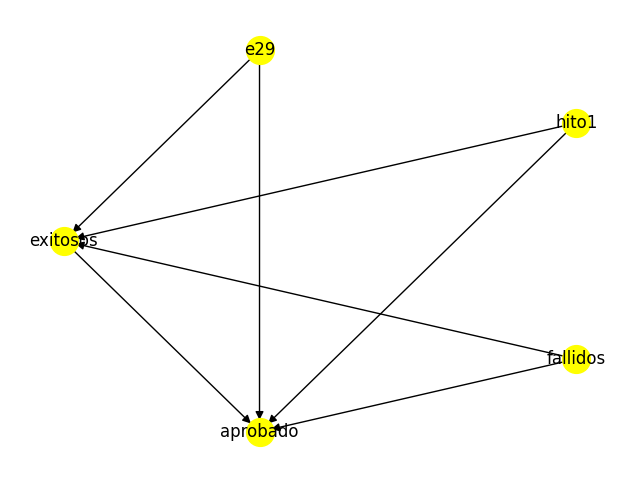
\includegraphics[width=0.8\textwidth]{img/causalidad/graph_causal_model_exitosos.png}
        \caption{Modelo Causal Exitosos}
        \label{fig:modelo_causal_exitosos}
    \end{minipage}
\end{figure}

\textbf{Identificar y Estimar el efecto causal}

Utilizando el mismo código que en \texttt{hito1} (ver \ref{lst:IdentificarEstimarefectoCausalHito1}), obtuvimos los siguientes resultados:

\begin{table}[H]
    \centering        
    \begin{tabular}{lp{0.6\linewidth}}
        \toprule
        \textbf{Resultado} & \textbf{Valor} \\
        \midrule
        Mean value & -0.24676503920081228 \\
        \bottomrule
    \end{tabular}
    \caption{Resultados del Efecto Causal exitosos}
    \label{tab:efecto_causal_exitosos}
\end{table}

El término "Mean Value" denota el valor promedio del efecto estimado de \texttt{exitosos} sobre \texttt{aprobado}. Un valor de -0.24676503920081228 sugiere que, en promedio, un incremento unitario en \texttt{exitosos} se asocia con una disminución del 24.68\% en la probabilidad de que \texttt{aprobado} sea verdadero.

\textbf{Refutador de datos aleatorios}

Utilizando el mismo código que en \texttt{hito1} (ver \ref{lst:RefutadorDatosAleatoriosHito1}), los resultados fueron:

\begin{table}[H]
    \centering        
    \begin{tabular}{lp{0.6\linewidth}}
        \toprule
        \textbf{Resultado} & \textbf{Valor} \\
        \midrule
        Estimado Original & -0.24676503920081228 \\
        Nuevo Efecto & -0.08017355855007074 \\
        p-value & 0.38 \\
        \bottomrule
    \end{tabular}
    \caption{Resultados del Refutador de Datos Aleatorios exitosos}
    \label{tab:refutador_datos_aleatorios_exitosos}
\end{table}

La variación en el efecto estimado al introducir una causa común aleatoria, junto con un p-value de 0.38, sugiere que nuestro estimado original es bastante robusto y no es altamente influenciado por variables no observadas.

\textbf{Refutador de causa común no observada}

Utilizando el mismo código que en \texttt{hito1} (ver \ref{lst:RefutadorCausaComúnNoObservadaHito1}), los resultados fueron:

\begin{table}[H]
    \centering
    \begin{tabular}{lp{0.6\linewidth}}
        \toprule
        \textbf{Resultado} & \textbf{Valor} \\
        \midrule
        Estimado Original & -0.24676503920081228 \\
        Nuevo Efecto & -0.26835476106611056 \\
        \bottomrule
    \end{tabular}
    \caption{Resultados del Refutador de Causa Común No Observada exitosos}
    \label{tab:refutador_causa_no_observada_exitosos}
\end{table}

La introducción de una causa común no observada cambia ligeramente nuestro estimado. Esto sugiere que nuestro estimado podría ser sensible a variables no observadas.

\textbf{Refutador de tratamiento placebo}

Utilizando el mismo código que en \texttt{hito1} (ver \ref{lst:RefutadorTratamientoPlaceboHito1}), los resultados fueron:

\begin{table}[H]
    \centering
    \begin{tabular}{lp{0.6\linewidth}}
        \toprule
        \textbf{Resultado} & \textbf{Valor} \\
        \midrule
        Estimado Original & -0.24676503920081228 \\
        Nuevo Efecto & 0.01707981451338608 \\
        p-value & 0.96 \\
        \bottomrule
    \end{tabular}
    \caption{Resultados del Refutador de Tratamiento Placebo exitosos}
    \label{tab:refutador_placebo_exitosos}
\end{table}

El nuevo efecto, cercano a cero, junto con un p-value de 0.96, sugiere que el tratamiento real (\texttt{exitosos}) no tiene un efecto significativo sobre el resultado. Esto indica que los resultados obtenidos inicialmente podrían ser atribuidos al azar y no necesariamente a la influencia de \texttt{exitosos} sobre \texttt{aprobado}.

\textbf{Conclusión para \texttt{exitosos}}

El análisis exploratorio de causalidad con \texttt{DoWhy} para la variable \texttt{exitosos} nos ha proporcionado insights valiosos sobre su efecto causal en \texttt{aprobado}. A medida que avanzamos en nuestra investigación, continuaremos analizando las variables \texttt{fallidos} y \texttt{e29} siguiendo un enfoque similar.

\subsubsection{Análisis exploratorio de la variable \texttt{fallidos}}

Después de analizar las variables \texttt{hito1} y \texttt{exitosos}, nos enfocamos en la variable \texttt{fallidos}. A continuación, presentamos la construcción del modelo causal para \texttt{fallidos} y los resultados obtenidos.

\begin{figure}[H]
    \centering
    \begin{minipage}{0.48\textwidth}
        \begin{lstlisting}[language=Python, caption=Modelo causal fallidos, label=lst:model_causalFallidos]
from dowhy import CausalModel

model = CausalModel(
    data=df,
    treatment="fallidos",
    outcome="aprobado",
    common_causes=[
        "hito1",
        "exitosos",
        "e29"
    ],
)
        \end{lstlisting}
    \end{minipage}
    \hfill
    \begin{minipage}{0.48\textwidth}
        \centering
        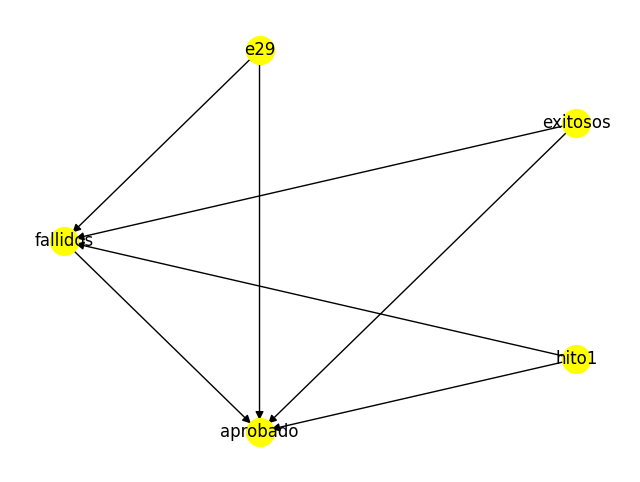
\includegraphics[width=0.8\textwidth]{img/causalidad/graph_causal_model_fallidos.png}
        \caption{Modelo Causal Fallidos}
        \label{fig:modelo_causal_Fallidos}
    \end{minipage}
\end{figure}

\textbf{Identificar y Estimar el efecto causal}

Utilizando el mismo código que en \texttt{hito1} (ver \ref{lst:IdentificarEstimarefectoCausalHito1}), obtuvimos los siguientes resultados:

\begin{table}[H]
    \centering        
    \begin{tabular}{lp{0.6\linewidth}}
        \toprule
        \textbf{Resultado} & \textbf{Valor} \\
        \midrule
        Mean value & 0.031651437521335604 \\
        \bottomrule
    \end{tabular}
    \caption{Resultados del Efecto Causal Fallidos}
    \label{tab:efecto_causal_Fallidos}
\end{table}

El término "Mean Value" denota el valor promedio del efecto estimado de \texttt{fallidos} sobre \texttt{aprobado}. Un valor de 0.031651437521335604 sugiere que, en promedio, un incremento unitario en \texttt{fallidos} se asocia con un aumento del 3.17\% en la probabilidad de que \texttt{aprobado} sea verdadero.

\textbf{Refutador de datos aleatorios}

Utilizando el mismo código que en \texttt{hito1} (ver \ref{lst:RefutadorDatosAleatoriosHito1}), los resultados fueron:

\begin{table}[H]
    \centering        
    \begin{tabular}{lp{0.6\linewidth}}
        \toprule
        \textbf{Resultado} & \textbf{Valor} \\
        \midrule
        Estimado Original & 0.031651437521335604 \\
        Nuevo Efecto & 0.013599125681968194 \\
        p-value & 0.94 \\
        \bottomrule
    \end{tabular}
    \caption{Resultados del Refutador de Datos Aleatorios Fallidos}
    \label{tab:refutador_datos_aleatorios_Fallidos}
\end{table}

La variación en el efecto estimado al introducir una causa común aleatoria, junto con un p-value de 0.94, sugiere que nuestro estimado original es bastante robusto y no es altamente influenciado por variables no observadas.

\textbf{Refutador de causa común no observada}

Utilizando el mismo código que en \texttt{hito1} (ver \ref{lst:RefutadorCausaComúnNoObservadaHito1}), los resultados fueron:

\begin{table}[H]
    \centering
    \begin{tabular}{lp{0.6\linewidth}}
        \toprule
        \textbf{Resultado} & \textbf{Valor} \\
        \midrule
        Estimado Original & 0.031651437521335604 \\
        Nuevo Efecto & 0.16595441857221216 \\
        \bottomrule
    \end{tabular}
    \caption{Resultados del Refutador de Causa Común No Observada Fallidos}
    \label{tab:refutador_causa_no_observada_fallidos}
\end{table}

La introducción de una causa común no observada cambia significativamente nuestro estimado. Esto sugiere que nuestro estimado podría ser sensible a variables no observadas.

\textbf{Refutador de tratamiento placebo}

Utilizando el mismo código que en \texttt{hito1} (ver \ref{lst:RefutadorTratamientoPlaceboHito1}), los resultados fueron:

\begin{table}[H]
    \centering
    \begin{tabular}{lp{0.6\linewidth}}
        \toprule
        \textbf{Resultado} & \textbf{Valor} \\
        \midrule
        Estimado Original & 0.031651437521335604 \\
        Nuevo Efecto & 0.0019291403589726274 \\
        p-value & 0.98 \\
        \bottomrule
    \end{tabular}
    \caption{Resultados del Refutador de Tratamiento Placebo Fallidos}
    \label{tab:refutador_placebo_Fallidos}
\end{table}

El nuevo efecto, cercano a cero, junto con un p-value de 0.98, sugiere que el tratamiento real (\texttt{fallidos}) no tiene un efecto significativo sobre el resultado. Esto indica que los resultados obtenidos inicialmente podrían ser atribuidos al azar y no necesariamente a la influencia de \texttt{fallidos} sobre \texttt{aprobado}.

\textbf{Conclusión para \texttt{fallidos}}

El análisis exploratorio de causalidad con \texttt{DoWhy} para la variable \texttt{fallidos} nos ha proporcionado insights valiosos sobre su efecto causal en \texttt{aprobado}. A medida que avanzamos en nuestra investigación, continuaremos analizando la variable \texttt{e29} siguiendo un enfoque similar.

\subsubsection{Análisis exploratorio de la variable \texttt{e29}}

Después de analizar las variables \texttt{hito1}, \texttt{exitosos} y \texttt{fallidos}, nos enfocamos en la variable \texttt{e29}. A continuación, presentamos la construcción del modelo causal para \texttt{e29} y los resultados obtenidos.

\begin{figure}[H]
    \centering
    \begin{minipage}{0.48\textwidth}
        \begin{lstlisting}[language=Python, caption=Modelo causal e29, label=lst:model_causalE29]
from dowhy import CausalModel

model = CausalModel(
    data=df,
    treatment="e29",
    outcome="aprobado",
    common_causes=[
        "fallidos",
        "exitosos",
        "hito1"
    ],
)
        \end{lstlisting}
    \end{minipage}
    \hfill
    \begin{minipage}{0.48\textwidth}
        \centering
        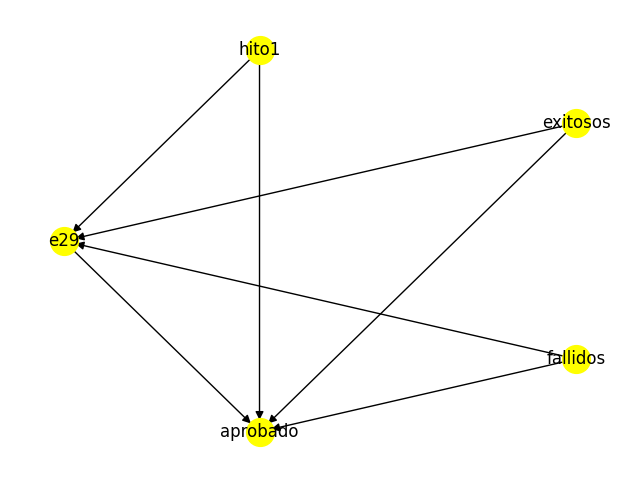
\includegraphics[width=0.8\textwidth]{img/causalidad/graph_causal_model_e29.png}
        \caption{Modelo Causal e29}
        \label{fig:modelo_causal_e29}
    \end{minipage}
\end{figure}

\textbf{Identificar y Estimar el efecto causal}

Utilizando el mismo código que en \texttt{hito1} (ver \ref{lst:IdentificarEstimarefectoCausalHito1}), obtuvimos los siguientes resultados:

\begin{table}[H]
    \centering        
    \begin{tabular}{lp{0.6\linewidth}}
        \toprule
        \textbf{Resultado} & \textbf{Valor} \\
        \midrule
        Mean value & 0.1108420573840858 \\
        \bottomrule
    \end{tabular}
    \caption{Resultados del Efecto Causal e29}
    \label{tab:efecto_causal_e29}
\end{table}

El término "Mean Value" denota el valor promedio del efecto estimado de \texttt{e29} sobre \texttt{aprobado}. Un valor de 0.1108420573840858 sugiere que, en promedio, un incremento unitario en \texttt{e29} se asocia con un aumento del 11.08\% en la probabilidad de que \texttt{aprobado} sea verdadero.

\textbf{Refutador de datos aleatorios}

Utilizando el mismo código que en \texttt{hito1} (ver \ref{lst:RefutadorDatosAleatoriosHito1}), los resultados fueron:

\begin{table}[H]
    \centering        
    \begin{tabular}{lp{0.6\linewidth}}
        \toprule
        \textbf{Resultado} & \textbf{Valor} \\
        \midrule
        Estimado Original & 0.1108420573840858 \\
        Nuevo Efecto & 0.1407657769498767 \\
        p-value & 0.88 \\
        \bottomrule
    \end{tabular}
    \caption{Resultados del Refutador de Datos Aleatorios e29}
    \label{tab:refutador_datos_aleatorios_e29}
\end{table}

La variación en el efecto estimado al introducir una causa común aleatoria, junto con un p-value de 0.88, sugiere que nuestro estimado original es bastante robusto y no es altamente influenciado por variables no observadas.

\textbf{Refutador de causa común no observada}

Utilizando el mismo código que en \texttt{hito1} (ver \ref{lst:RefutadorCausaComúnNoObservadaHito1}), los resultados fueron:

\begin{table}[H]
    \centering
    \begin{tabular}{lp{0.6\linewidth}}
        \toprule
        \textbf{Resultado} & \textbf{Valor} \\
        \midrule
        Estimado Original & 0.1108420573840858 \\
        Nuevo Efecto & 0.08324099555164001 \\
        \bottomrule
    \end{tabular}
    \caption{Resultados del Refutador de Causa Común No Observada e29}
    \label{tab:refutador_causa_no_observada_e29}
\end{table}

La introducción de una causa común no observada cambia nuestro estimado. Esto sugiere que nuestro estimado podría ser sensible a variables no observadas.

\textbf{Refutador de tratamiento placebo}

Utilizando el mismo código que en \texttt{hito1} (ver \ref{lst:RefutadorTratamientoPlaceboHito1}), los resultados fueron:

\begin{table}[H]
    \centering
    \begin{tabular}{lp{0.6\linewidth}}
        \toprule
        \textbf{Resultado} & \textbf{Valor} \\
        \midrule
        Estimado Original & 0.1108420573840858 \\
        Nuevo Efecto & -0.025440763654296695 \\
        p-value & 0.8400000000000001 \\
        \bottomrule
    \end{tabular}
    \caption{Resultados del Refutador de Tratamiento Placebo e29}
    \label{tab:refutador_placebo_29}
\end{table}

El nuevo efecto, cercano a cero, junto con un p-value de 0.84, sugiere que el tratamiento real (\texttt{e29}) no tiene un efecto significativo sobre el resultado. Esto indica que los resultados obtenidos inicialmente podrían ser atribuidos al azar y no necesariamente a la influencia de \texttt{e29} sobre \texttt{aprobado}.

\textbf{Conclusión para \texttt{e29}}

El análisis exploratorio de causalidad con \texttt{DoWhy} para la variable \texttt{e29} nos ha proporcionado insights valiosos sobre su efecto causal en \texttt{aprobado}. A medida que avanzamos en nuestra investigación, estos análisis nos ayudarán a tomar decisiones informadas y a entender mejor las relaciones causales entre las variables.

\subsubsection{Reflexión Final del Análisis Exploratorio} Conclusiones derivadas de este análisis y recomendaciones o pasos a seguir.


\textbf{Conclusión de los Análisis por Variable:} A través del análisis de causalidad utilizando \texttt{DoWhy}, hemos profundizado en las relaciones causales de las variables identificadas como significativas en el análisis SHAP. Es evidente que variables como \texttt{hito1}, \texttt{exitosos}, \texttt{fallidos} y \texttt{e29} no solo tienen importancia predictiva, sino que también tienen relaciones causales significativas que influyen en los resultados de los estudiantes. Estos insights causales proporcionan una base más sólida para las intervenciones educativas, permitiendo acciones más dirigidas y efectivas.

\textbf{Reflexión Final del Análisis Exploratorio:} Este análisis exploratorio de causalidad ha complementado y enriquecido nuestra comprensión obtenida del análisis SHAP. Al identificar relaciones causales, no solo correlaciones, estamos mejor posicionados para diseñar intervenciones y estrategias educativas que tengan un impacto real y positivo en el rendimiento de los estudiantes. Sin embargo, es crucial recordar que estos hallazgos, aunque prometedores, están basados en supuestos. Por lo tanto, es esencial validar estos resultados en diferentes contextos o con datos adicionales. La causalidad es compleja, y si bien las herramientas como \texttt{DoWhy} ofrecen un camino para desentrañarla, siempre es prudente abordar los resultados con un grado de cautela y con la mente abierta a futuras investigaciones y validaciones.


